\chapter{Implementacja}

\section{Architektura}

%TODO zarys architektóry


%TODO opis API dostarczanego przez aplikacje serwerową w tabelce 



\section{Aplikacja serwerowa}
Do zarządzania danymi wykorzystywana jest aplikacja serwerowa. Przetwarza ona żądania aplikacji klienckiej. Dostarcza ona funkcjonalność uwierzytelniania i autoryzacji. W wyniku zapytań wysłanych przez aplikację kliencką wyświetlane są w aplikacji odpowiednie dane. Możliwe jest też dodawanie i usuwanie odpowiednich rekordów. Implementacja odbywa się z wykorzystywaniem języka Java z frameworkami Spring oraz Hibernate \ref{tab:zestawienie_narzędzi}

\subsection{Struktura projektu}
Ścieżka pakietowa wykorzystana jest odwróconą ścieżką domenową Politechniki Wrocławskiej oraz nazwy projektu: pl.pwr.edu.computermanagamenttool. Następnie pakiety które są dołączone do tej ścieżki odpowiadają funkcjom które pełnią klasy. Wyróżnia się tutaj:


\begin{figure}[htb]
  \centering
	\begin{tabular}{@{}lll@{}}
	a) & b) & c) \\
  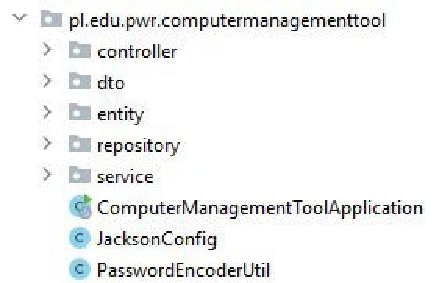
\includegraphics[width=0.3\textwidth]{rys05/ogolne.pdf} & 
	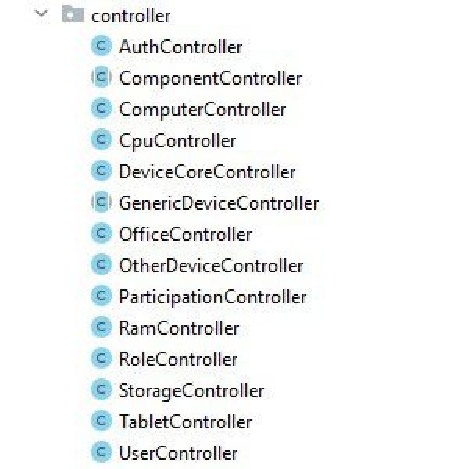
\includegraphics[width=0.3\textwidth]{rys05/controller.pdf} &
	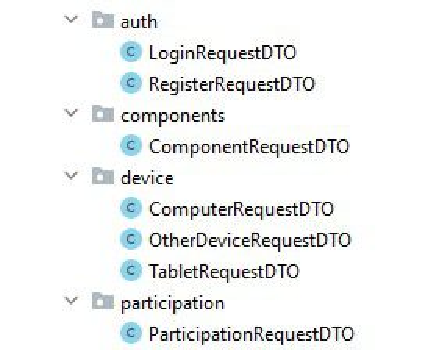
\includegraphics[width=0.3\textwidth]{rys05/dto.pdf} \\

	d) & e) & f) \\
	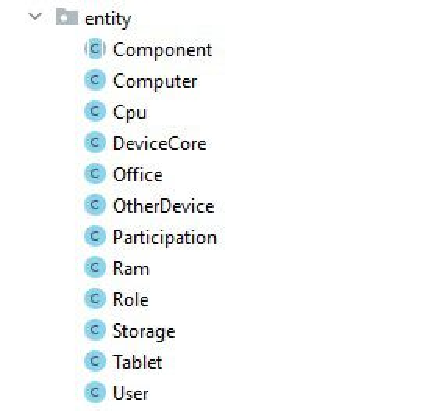
\includegraphics[width=0.3\textwidth]{rys05/entity.pdf} &
	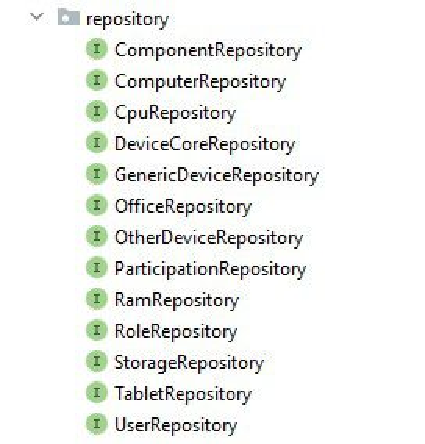
\includegraphics[width=0.3\textwidth]{rys05/repository.pdf} &
	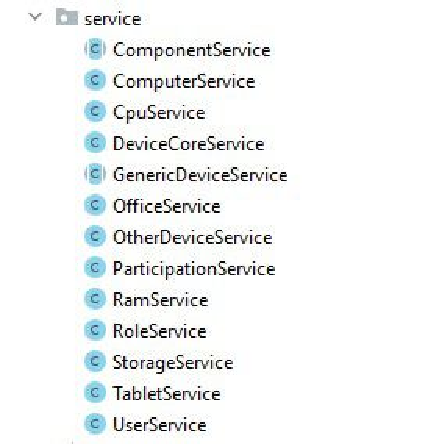
\includegraphics[width=0.3\textwidth]{rys05/service.pdf}
	\end{tabular}
  \caption{Struktura projektu a) ogólna struktura, b) kontrolery, c) data transfer object, d) encje, e) repozytoria, f) serwisy}
  \label{backend_struktura:label}
\end{figure}

\subsection{Fragmenty implementacji}
\subsubsection {Przykład encji wykorzystującej schemat dziedziczenia}

\begin{lstlisting}[language=Java, style=JavaStyle, caption={Fragment klasy nadrzędnej DeviceCore}, label={entity_deviceCore}]
@Entity
@Table(name = "device_core")
@Inheritance(strategy = InheritanceType.TABLE_PER_CLASS)
public class DeviceCore {
    @Id
    @GeneratedValue(strategy = GenerationType.TABLE)
    @Column(name = "id", nullable = false)
    private Integer id;

    @Column(name = "device_type", length = 50)
    private String deviceType;

    @Column(name = "device_name", length = 50)
    private String deviceName;

\end{lstlisting}


\begin{lstlisting}[language=Java, style=JavaStyle,  caption={Fragment klasy potomnej Computer}, label={entity_computer}]
@Entity
@Table(name = "computer")
public class Computer extends DeviceCore{

    public static final String DEVICE_TYPE = "COMPUTER";
    @Column(name = "serial_number", length = 50)
    private String serialNumber;

    @Column(name = "operating_system", length = 50)
    private String operatingSystem;

    @Column(name = "battery_life", length = 50)
    private String batteryLife;
		
		@ManyToOne(fetch = FetchType.EAGER)
    @JoinColumn(name = "cpu_id")
    private Cpu cpu;

\end{lstlisting}


\subsubsection{Przykład repozytorium dla wszystkich urządzeń}
Repozytorium sprzętu komputerowego zostało napisane z użyciem wyrażeń generycznych. Wykorzystanie ich przyczynia się do uproszczenia kodu oraz łatwiejszej jego rozbudowy.

\begin{lstlisting}[language=Java, style=JavaStyle,  caption={Generyczne repozytorium sprzętu komputerowego}, label={repo_genericDevice}]
@NoRepositoryBean
public interface GenericDeviceRepository<T extends DeviceCore> extends JpaRepository<T, Integer> {

    List<T> findAllByReadyToSellIsTrue();
    List<T> findAllByReadyToSellIsFalse();
    List<T> findAllByOfficeId(int officeId);
}
\end{lstlisting}

W lini 1 adnotacja @NoRepositoryBean jest używana do oznaczenia interfejsów które nie mają mieć swojej instancji. Oznacza to, że nie jest on przeznaczony do utworzenia instancji repozytorium w trakcie uruchomiania aplikacji. Z racji tego że klasy sprzętu komputerowego mają zbliżone funkcjonalności nie trzeba dostarczać tych samych interfejsów we wszystkich repozytoriach tylko zastosować schemat dziedziczenia. To samo dotyczy się kontrolerów co pokazano w następnym podrozdziale.

\subsubsection{Kontroler sprzętu komputerowego}

\begin{lstlisting}[language=Java, style=JavaStyle,  caption={Wybrane metody generycznego kontrolera sprzętu komputerowego}, label={controller_genericDevice}]
@GetMapping("/all")
 List<T> getAllBasicDevices(){
 return genericDeviceService.getAllDevices();
} 
@DeleteMapping("/{id}")
void deleteDevice(@PathVariable int id){
genericDeviceService.deleteDevice(id);
}

@PutMapping("/set-ready-to-lottery/{id}")
@CrossOrigin(origins = "*")
public ResponseEntity<T> setReadyToLottery(@PathVariable int id){
    try{
        T updatedBasicDevice = genericDeviceService.setReadyToLottery(id);
        return new ResponseEntity<>(updatedBasicDevice, HttpStatus.OK);
    } catch (RuntimeException e){
        return new ResponseEntity<>(HttpStatus.NOT_FOUND);
    }
}
\end{lstlisting}

Powyższy Listing kodu \ref{repo_genericDevice} umożliwia jednym zapytaniem uzyskanie wszystkich danych dotyczące urządzeń, wliczając to także dane które są unikalne dla klas potomnych. Dzięki temu można zestawić w tabeli a aplikacji klienckiej ogólne informacje dotyczące sprzętu. Zastosowano mechanizm dziedziczenia, dzięki czemu klasy dziedziczące po generycznym repozytorium umożliwiają uzyskanie tylko danych sprzętów należących do kategorii klasy potomnych. Aby uzyskać właśnie tylko sprzęty klasy potomnej wystarczy zmienić tylko endpoint i nie jest konieczne powielanie kodu. Klasy dziedziczące rozszerzają funkcjonalność generycznego repozytorium dodając metody unikalne dla wybranego sprzętu.

\subsubsection{Dodawanie tabletu przy wykorzystaniu rdzenia sprzętu}
Wszystkie klasy potomne mają wspólne atrybuty dlatego wykorzystano generyczny serwis by zredukować powielenie kodu

\begin{lstlisting}[language=Java, style=JavaStyle,  caption={Dodawanie Tabletu z wykorzystaniem klasy nadrzędnej}, label={service_tablet}]
protected DeviceCore addDevice(Class<? extends DeviceCore> deviceClass, String deviceName, Double price, String description, Integer age, Boolean readyToSell, Integer officeId) {

        if(officeId == null){
            throw new RuntimeException("Office required");
        }
        Optional<Office> officeOptional = officeRepository.findById(officeId);
        Office office = officeOptional.orElseThrow(() -> new RuntimeException("Office not found with id: " + officeId));

        DeviceCore deviceCore;
        try {
            deviceCore = deviceClass.getDeclaredConstructor().newInstance();
        } catch (InstantiationException | IllegalAccessException | NoSuchMethodException | InvocationTargetException e) {
            throw new RuntimeException("Error creating device", e);
        }

        deviceCore.setDeviceName(deviceName);
        deviceCore.setPrice(price);
        deviceCore.setDescription(description);
        deviceCore.setAge(age);
        deviceCore.setReadyToSell(readyToSell);
        deviceCore.setOffice(office);

        return deviceCore;
    }

public Tablet addTablet(String deviceName, Double price, String description,
                            Integer age, Boolean readyToSell, Integer officeId,
                            String screenSize, String operatingSystem, String batteryLife){

        Tablet tablet = (Tablet) addDevice(Tablet.class, deviceName, price, description,
                                                                age, readyToSell, officeId);

        tablet.setScreenSize(screenSize);
        tablet.setOperatingSystem(operatingSystem);
        tablet.setBatteryLife(batteryLife);

        return genericDeviceRepository.save(tablet);
    }

\end{lstlisting}

W Listingu \ref{service_tablet} metoda w linii 1 z klasy generycznej oprócz atrybutów pól przyjmuję też jako argument obiekt typu Class. Wykorzystywany jest on w linii 11 do stworzenia instancji klasy. Dzięki temu we wszystkich klasach potomnych, wspólne atrybuty są ustawiane przez klasę nadrzędną(linie 16-21). Przykład ustawiania unikalnych pól klasy podrzędnej są w liniach 33-35.


\section {Aplikacja kliencka}
%TODO wstęp

\subsection{Struktura projektu}


\subsection{Fragmenty implementacji}
\subsubsection{Widoki aplikacji}
%TODO opisy scieżek w aplikacji
\subsubsection{Renderowanie danych w tabeli}

\subsection{Instrukcja użytkowania}
\subsubsection{Logowanie i rejestracja}

\subsubsection{Administrator}
\subsubsection{Pracownik}



